
%(BEGIN_QUESTION)
% Copyright 2006, Tony R. Kuphaldt, released under the Creative Commons Attribution License (v 1.0)
% This means you may do almost anything with this work of mine, so long as you give me proper credit

Determine the voltmeter's indication in this thermocouple circuit (type J) for the following temperatures:

$$\includegraphics[width=15.5cm]{i00380x01.eps}$$

\begin{itemize}
\item{} $T_{measurement}$ = 250$^{o}$ F ; $T_{reference}$ = 60$^{o}$ F ; Voltmeter voltage = ??? 
\item{} $T_{measurement}$ = 733$^{o}$ F ; $T_{reference}$ = 72$^{o}$ F ; Voltmeter voltage = ??? 
\item{} $T_{measurement}$ = $-$60$^{o}$ F ; $T_{reference}$ = 49$^{o}$ F ; Voltmeter voltage = ??? 
\item{} $T_{measurement}$ = $-$238$^{o}$ F ; $T_{reference}$ = 80$^{o}$ F ; Voltmeter voltage = ??? 
\end{itemize}

\vskip 20pt \vbox{\hrule \hbox{\strut \vrule{} {\bf Suggestions for Socratic discussion} \vrule} \hrule}

\begin{itemize}
\item{} Students often get confused regarding the mathematical relationship between measurement junction voltage and reference junction voltage.  Do these voltages aid each other (add), or do they oppose each other (subtract)?  Devise a simple ``thought experiment'' whereby you may prove to yourself which of these stated relationships is correct.
\end{itemize}

\underbar{file i00380}
%(END_QUESTION)





%(BEGIN_ANSWER)

\noindent
{\bf Partial answer:}

\begin{itemize}
\item{} $T_{measurement}$ = 250$^{o}$ F ; $T_{reference}$ = 60$^{o}$ F ; Voltmeter voltage = 5.630 mV 
%\item{} $T_{measurement}$ = 733$^{o}$ F ; $T_{reference}$ = 72$^{o}$ F ; Voltmeter voltage = 20.132 mV 
%\item{} $T_{measurement}$ = $-$60$^{o}$ F ; $T_{reference}$ = 49$^{o}$ F ; Voltmeter voltage = $-$2.961 mV
\item{} $T_{measurement}$ = $-$238$^{o}$ F ; $T_{reference}$ = 80$^{o}$ F ; Voltmeter voltage = $-$7.864 mV
\end{itemize}

%(END_ANSWER)





%(BEGIN_NOTES)

(From ITS-90 thermocouple table:)

\begin{itemize}
\item{} $T_{measurement}$ = 250$^{o}$ F ; $T_{reference}$ = 60$^{o}$ F ; Voltmeter voltage = 5.630 mV 
\item{} $T_{measurement}$ = 733$^{o}$ F ; $T_{reference}$ = 72$^{o}$ F ; Voltmeter voltage = 20.132 mV 
\item{} $T_{measurement}$ = $-$60$^{o}$ F ; $T_{reference}$ = 49$^{o}$ F ; Voltmeter voltage = $-$2.961 mV
\item{} $T_{measurement}$ = $-$238$^{o}$ F ; $T_{reference}$ = 80$^{o}$ F ; Voltmeter voltage = $-$7.864 mV
\end{itemize}





\vfil \eject

\noindent
{\bf Summary Quiz:}

Referencing a table of millivoltage values for type K thermocouples (ITS-90), determine the amount of millivoltage seen by a meter connected to a type K thermocouple assuming a measurement junction temperature of 295 $^{o}$F and a reference junction temperature of 68 $^{o}$F.

\begin{itemize}
\item{} 0.798 mV
\vskip 5pt 
\item{} 5.184 mV
\vskip 5pt 
\item{} 5.318 mV
\vskip 5pt 
\item{} 6.780 mV
\vskip 5pt 
\item{} 6.049 mV
\vskip 5pt 
\item{} 5.982 mV
\end{itemize}





\vfil \eject

\noindent
{\bf Summary Quiz:}

Referencing a table of millivoltage values for type J thermocouples (ITS-90), determine the amount of millivoltage seen by a meter connected to a type J thermocouple assuming a measurement junction temperature of 502 $^{o}$F and a reference junction temperature of 69 $^{o}$F.

\begin{itemize}
\item{} 15.220 mV
\vskip 5pt 
\item{} 1.048 mV
\vskip 5pt 
\item{} 14.172 mV
\vskip 5pt 
\item{} 13.523 mV
\vskip 5pt 
\item{} 13.124 mV
\vskip 5pt 
\item{} 13.062 mV
\end{itemize}


%INDEX% Measurement, temperature: thermocouple

%(END_NOTES)


